\documentclass[UTF8,a4paper,10pt,fontset=fandol]{ctexart}
\usepackage[top=1.8cm,bottom=1.8cm,left=2cm,right=2cm]{geometry}
\usepackage{tabularx,booktabs,array,enumitem,xcolor,fancyhdr,fvextra,hyperref,xurl,graphicx}
\hypersetup{colorlinks=true,urlcolor=blue,pdftitle={CampusClaw 个人 AI 应用平台验证报告},pdfauthor={CampusClaw 个人项目}}
\pagestyle{fancy}\fancyhf{}\fancyhead[L]{\small CampusClaw｜个人项目功能验收}\fancyhead[R]{\small 2026-10-21}\fancyfoot[C]{\thepage}
\setlength{\headheight}{14pt}\setlength{\parindent}{2em}\setlength{\parskip}{0.35em}\setlength{\emergencystretch}{2em}
\setlist{leftmargin=1.7em,itemsep=0.2em,topsep=0.25em}
\newcolumntype{Y}{>{\raggedright\arraybackslash}X}
\newcommand{\code}[1]{\texttt{\detokenize{#1}}}
\fvset{breaklines=true,breakanywhere=true,fontsize=\footnotesize}
\begin{document}
\begin{center}
{\LARGE\bfseries CampusClaw 个人 AI 应用平台验证报告}\\[0.6em]
{\large 功能补齐后的复验与 LLM 调用证据}\\[0.5em]
2026 年 10 月 21 日 · 个人项目阶段
\end{center}
\section*{1. 项目简介与验收结论}
CampusClaw 是面向课程学习的个人 AI 应用平台。用户可使用写作润色、学习规划、练习生成与课程资料问答，组合提示词模板、声明式 Skill、班级知识库以及外部工具。教师维护本班模板、资料和技能并启用连接，学生在授权范围内使用；新应用执行记录仅本人可见。

Git 仓库：\href{https://github.com/lezhonglezhong/campusclaw-freebird}{github.com/lezhonglezhong/campusclaw-freebird}。本次基于本地 Git 和实际部署验证，不以远端仓库公开可访问性作为验收依据。运行代码提交基线为 \code{6a6f8f1}；后续提交补充报告、阶段文档及归档规格。证据同时保存部署运行文件哈希，便于确定实际代码版本。

技术栈：Flask、SQLAlchemy、MySQL 8、Qdrant、原生 JavaScript；Docker Compose 部署。模型使用 OpenAI-compatible Chat Completions 和 Embeddings 接口，当前模型分别为 course-chat 与 course-embedding。页面通过 sessionStorage 中的 JWT 发起 Bearer 请求，不使用 Cookie 登录。

\textbf{复验结论：题目要求的五类平台能力均已实现，在本报告明确的格式、协议和验证范围内通过验收。}此前的功能缺项已补齐；结论不扩展为支持任意技能格式、所有 MCP 版本或生产级性能保证。

\noindent\begin{tabularx}{\linewidth}{p{3.1cm}p{1.8cm}Y}
\toprule
要求 & 复验 & 可操作的交付能力\\\midrule
多个 AI 应用 & 通过 & 工作台三个独立应用及既有知识问答；各有不同系统指令与输出目的。\\
提示词模板 & 通过 & 教师保存、编辑、删除；班级内选用；变量替换和发送前预览。\\
知识库检索 & 通过 & 关键词/向量/混合检索；新应用可绑定本班知识；有限切片及引用校验。\\
内置及上传 Skill & 通过 & 两个内置技能；16 KiB 以内 JSON 上传；1–3 个模型步骤顺序执行。\\
外部工具与 MCP & 通过 & HTTP JSON 工具、MCP 2025-06-18 Streamable HTTP；真实工具调用与结果回填。\\\bottomrule
\end{tabularx}

入口：\code{/apps} 为新工作台，\code{/materials} 保留原有资料与问答。默认演示 HTTP/MCP 计算器由独立内部服务提供；教师先启用连接，用户再勾选允许本次使用的工具。外部服务地址和凭据由部署者在服务器配置。

\textbf{个人阶段成果复用：}现有应用、模板、知识库、Skill、工具接入、执行记录及验证材料均已完成。后续只需针对尚未实现的教学业务增量另行规划，不重复建设这些基础能力。

\newpage
\section*{2. 验证方式与证据范围}
\noindent\begin{tabularx}{\linewidth}{p{3.1cm}Y}
\toprule
验证层 & 方法与实际结果\\\midrule
自动化回归 & 全量 \textbf{226 项 pytest 测试通过}，包括原有 168 项和本次新增 58 项。逐项任务按仓库规则两次验证后分别提交。\\
真实浏览器 & Chromium 实际登录、模板新建/编辑/删除、技能上传/选择/删除、MCP 启用、运行与记录查看；另验证学生只读、匿名跳转、手机宽度及退出登录。模型为确定性替身。\\
受控 HTTP 采集 & 10 组场景通过。真实 API、HTTP 序列化和独立 HTTP/MCP 工具服务；模型返回受控。完整内容见 platform-controlled.json。\\
真实模型复验 & 使用容器私有网关配置，对隔离临时数据运行相同 10 组场景；真实 HTTP/MCP 工具，完整模型请求/响应见 platform-live.json。\\
部署检查 & 应用、MySQL、Qdrant、demo-tools 均 healthy；新接口、登录及材料读取通过；匿名应用目录为 401。现有数据卷与私有配置保留。\\\bottomrule
\end{tabularx}

真实模型复验包含三个应用、选定模板、内置技能、上传技能、知识绑定、HTTP 工具、MCP 工具和无证据分支。知识绑定复验采用隔离 SQLite、合成材料及可控向量候选；不是将线上全文或真实学生资料导出后测试。原有真实嵌入调用已确认 2048 维；新部署冒烟确认现有服务可用。

\textbf{证据目录：}\path{docs/verification/}。platform-controlled.json 和 platform-live.json 保存每组客户端输入、API 返回、完整运行记录与运行文件 SHA-256；platform-deployment.json 保存部署接口状态；workspace.png 为受控浏览器验收截图。模型密钥、用户 JWT、服务鉴权头和私有连接地址均不写入执行记录。

\subsection*{复现入口}
\begin{Verbatim}[frame=single]
python -m pip install -r requirements-dev.txt
python -m playwright install chromium
PYTHONDONTWRITEBYTECODE=1 python -m pytest -q -p no:cacheprovider
PYTHONDONTWRITEBYTECODE=1 python docs/verification/capture_platform.py
# 以下实际消耗模型额度，但仅使用临时合成资料
 docker compose exec -T campusclaw python docs/verification/capture_platform.py --live
PYTHONDONTWRITEBYTECODE=1 python docs/verification/verify_platform_report.py
\end{Verbatim}

\subsection*{验证限制}
首次真实学习规划场景返回 503，记录显示已发送请求但未收到网关响应；部署模型请求超时由默认 10 秒调为 30 秒后复测通过。知识绑定复测使用更明确的“仅复述资料事实”输入，返回“光合作用需要阳光[1]”。初测与复测 JSON 均保留，最终 platform-live.json 汇总各场景最近的验证结果。

真实模型样本代表本次运行，不保证后续生成文本逐字一致。MCP 验证覆盖选定版本、JSON/SSE、会话、分页及独立演示服务；未对所有第三方服务逐一认证。没有开展高并发压测、长期质量实验或完整渗透测试；不将这些未做的工作计入通过项。

\newpage
\section*{3. 问题一：发送的具体参数、提示词与返回}
\subsection*{3.1 两条业务入口}
原有页面向 \code{POST /api/ask} 发送 question；API 可接收受限 user/assistant 历史，页面本身不发送历史。新工作台向 \code{POST /api/platform/runs} 发送 app\_id、input、audience、template\_id、skill\_id、use\_knowledge、tools；这些字段由服务端校验和解析，不原样作为模型顶层参数。

用户 JWT 只用于访问应用。模型 HTTP 请求为 POST，Content-Type 为 application/json，Authorization 为服务器网关密钥；请求地址为配置基址后追加 \code{/chat/completions}。无工具时正文仅为 model 和 messages；有选定工具时增加 tools 与 tool\_choice=auto。不显式设置 temperature、top\_p、max\_tokens 或 stream；当前按完整 JSON 响应处理。

\subsection*{3.2 实际无工具请求正文}
以下直接取自本次真实模型 writing 场景第一轮请求，长行仅为排版折行：
\VerbatimInput[frame=single]{docs/verification/platform-sample-request.json}

\textbf{模板会一并发送。}新应用先替换 input/audience 变量，结果写入 user 消息的 Rendered template 部分，应用专用规则位于 system 消息。自定义模板会覆盖默认模板文本，不覆盖服务端权限和工具允许列表；变量值只作一次字面替换，不执行 Jinja 或代码。

\subsection*{3.3 返回内容}
网关返回的完整 JSON 保存在每个 exchange.response。生成路径读取 choices[0].message：有 tool\_calls 时执行工具循环，否则使用非空 content。模型返回的 id、usage、reasoning\_content 等附加字段不保证始终存在；这些字段可在本人折叠的详细运行记录中检查，不当作最终答案。

新 API 返回 answer、citations、run\_id、status；失败时返回稳定 error 与 run\_id。旧 \code{/api/ask} 仍只返回 answer/citations，并仅消费 content，不增加新工作台工具流程。本次 writing 的真实最终 content 全文如下（网关其余返回字段及 API 包装见配套 JSON）：
\VerbatimInput[frame=single]{docs/verification/platform-sample-answer.txt}

\newpage
\section*{4. 问题二：知识库是否每次完整发送？}
\textbf{不会自动把整库正文发给对话模型。}新工作台的“绑定本班知识库”开关按次生效；班级由当前数据库用户决定，客户端不能通过 class\_id 获取其他班资料。关闭开关时，新应用不执行知识检索。

\begin{enumerate}
\item 绑定知识库后按当前输入检索；新应用使用输入的前 500 字符作为查询，完整用户输入仍参与生成。旧问答的问题本身上限为 500 字符。
\item 混合检索执行关键词与向量检索，向量结果最低相似度为 0.35；向量服务先按班级过滤，关系数据库回查再次检查班级与索引状态。
\item RRF 融合（k=60）后，问答候选池最多 12 条；去重、按问题词项筛选，一般最多 4 个证据切片，比较题最多 8 个；无法区分时回退最多 4 个。
\item 仅这些切片的标题、序号及完整切片正文以 Sources 写入模型消息。返回卡片摘要最多 240 字符，但模型收到的是被选切片全文。
\item 无证据时直接返回“资料中未找到相关内容”，不调用 Chat。最终有知识来源的答案须通过引用/数字校验，必要时纠正一次，仍失败则返回 503。
\end{enumerate}

若一份短材料只有一个切片，选中它可能发送该材料全文；极小知识库也可能全部被命中。准确结论是“检索后发送有界证据”，不是“任何材料全文都绝不外发”。模型检查只能验证引用与部分数值关系，不能替代人工语义正确性判断。

\subsection*{建索引与问答是不同阶段}
上传/重建索引时，各切片逐一请求：
\begin{Verbatim}[frame=single]
POST <EMBEDDING_BASE_URL>/embeddings
{"model":"course-embedding","input":["当前切片完整正文"]}
\end{Verbatim}
因此材料的全部正文可能分多次发送给嵌入服务。问答检索阶段则将当前查询写入 input，不重新发送全部材料。2048 维是本地向量校验及建库配置，不作为 dimensions 参数发送。Qdrant 保存向量和来源标识，正文保存在关系数据库。

\subsection*{本次证据}
合成材料“光合作用需要阳光。”用于知识绑定样本。运行记录能检查 sources 及 Sources 消息；无证据样本 exchanges 为空。已有跨班隔离、去重、比较题证据筛选及错误引用重试测试继续通过。关键词匹配可能在本地读取本班全部 ready 切片，这是本地处理，不等同于外发全库；大库性能仍需独立压测。

定位：\path{campusclaw/platform_execution.py}、\path{campusclaw/knowledge_api.py}、\path{campusclaw/knowledge_retrieval.py}、\path{campusclaw/knowledge_indexing.py}。

\newpage
\section*{5. 问题三、四：Skill 内容与执行逻辑}
\textbf{当前支持的技能是声明式 JSON 模型工作流。}两个内置技能为“起草与审校”“学习教练”，教师可上传班级技能，学生可选用。文件最多 16 KiB，固定 version/name/description/instructions/steps 字段；步骤仅有 name 和 instruction，共 1–3 步。不支持任意脚本、ZIP 技能包、SKILL.md 附带资源或 shell 执行。

\subsection*{5.1 是否发送全部技能内容？}
\textbf{是。每个模型步骤都会把整个已校验 JSON 清单写入 system 消息。}包括名称、描述、总指令和全部步骤，同时另写当前步骤指令；不是只传技能名称，也不是按需读取一个片段。因为格式不包含脚本/附件，“全部内容”在这里指被支持并通过校验的完整清单。

页面示例可上传文件内容如下；真实上传场景以同样格式执行：
\VerbatimInput[frame=single]{campusclaw/static/example-skill.json}

\subsection*{5.2 实际执行顺序}
\begin{enumerate}
\item 验证用户、班级、文件/模板引用与工具选择，读取技能快照；无权限在调用模型前拒绝。
\item 为第一个步骤组装应用指令、完整清单、当前步骤、输入、已渲染模板和可选有限知识证据，调用模型。
\item 如有合法工具请求，执行选定工具并回填结果，再继续该步骤。
\item 第二个及之后的步骤接收上一步输出，重新包含完整清单和相同用户/模板/知识上下文；按步骤顺序执行。
\item 最后一步结果成为候选答案；绑定知识库时继续做引用校验。每一步的状态和输出、每轮模型请求/响应、工具调用均保存到本人执行记录。
\end{enumerate}

任一步模型失败会立即停止后续步骤并标记运行失败。单次最多 4 次工具调用、每步骤最多 3 轮模型请求；最终引用不合格可额外纠正一次。真实内置及上传样本各完成两个步骤，受控测试还覆盖上传格式错误、越班访问和失败中断。

定位：\path{campusclaw/platform_skills.py}、\path{campusclaw/platform_execution.py}；完整清单在每个真实样本的 trace.skill 与 exchange.request.messages[0] 中可对照。

\newpage
\section*{6. 问题五：MCP 接入后的模型参数与调用链}
模型仍调用 Chat Completions，不直接与 MCP 服务器对话。后端先进行 MCP initialize、notifications/initialized 和 tools/list，把选定工具映射成 OpenAI-compatible function 定义。以下为本次真实 MCP 场景发送给模型的 tools 中一项：
\VerbatimInput[frame=single]{docs/verification/platform-sample-tool.json}

\textbf{第一轮模型请求：}model、messages、tools（只包含用户选中工具）、tool\_choice=auto。模型返回 assistant.tool\_calls，function.name 是映射后的名称，arguments 是 JSON 字符串。本次工具参数为 a=13、b=17、operation=multiply。

\textbf{实际外部调用：}后端校验 JSON Schema 后，将映射名还原为 MCP 原始工具名 calculate；发送 JSON-RPC tools/call，params 为 name=calculate 和 arguments 对象。服务器返回 content/structuredContent，结果为 221。HTTP 工具场景则 POST 相同参数到部署配置的固定 JSON 接口。

\textbf{第二轮模型请求：}保留已有 system/user 消息，并追加原始 assistant.tool\_calls，随后追加 role=tool、tool\_call\_id 与对应 JSON 结果。模型依据实际工具结果生成最终回答。完整两轮及真实返回见 platform-live.json 的 mcp\_tool/http\_tool 场景；没有把工具实现源码、服务器配置或鉴权凭据塞入提示词。

\textbf{协议和限制：}支持 MCP 2025-06-18 Streamable HTTP 的 JSON/POST SSE 返回、会话头、版本头和有界分页；不支持 stdio、OAuth 配置、sampling 或其他版本的全部扩展。未知工具、重复调用 ID、错误参数、上游错误及超额调用均失败，不伪装为成功。

规范依据：\href{https://modelcontextprotocol.io/specification/2025-06-18/basic/transports}{MCP transports}、\href{https://modelcontextprotocol.io/specification/2025-06-18/basic/lifecycle}{lifecycle}、\href{https://modelcontextprotocol.io/specification/2025-06-18/server/tools}{tools}。实现定位：\path{campusclaw/platform_tools.py}、\path{campusclaw/platform_chat.py}。

\newpage
\section*{7. 测试矩阵与可追溯交付}
\noindent\begin{tabularx}{\linewidth}{p{4cm}p{1.7cm}Y}
\toprule
任务或场景 & 结果 & 证据\\\midrule
应用目录与模板 & 9 通过 & 三应用、模板 CRUD、变量安全替换、班级及教师权限。\\
声明式 Skill & 10 通过 & 内置/上传、格式/大小检查、顺序执行、完整清单和失败中断。\\
HTTP/MCP 适配与工具循环 & 17 通过 & 实际本机 HTTP/SSE、握手、分页、会话、参数、未知工具和限额。\\
统一执行与私有记录 & 18 通过 & 应用指令、选定模板/技能、工具回填、知识引用及记录访问隔离。\\
浏览器与演示服务 & 4 通过 & Chromium 桌面/手机流程、教师管理和学生只读；演示协议及错误返回。\\
原有回归 & 168 通过 & 认证、班级隔离、材料、检索、知识问答等保持通过。\\\midrule
全量 & 226 通过 & 全量 pytest 无失败；逐任务验证后提交。\\
受控/真实场景 & 各 10 通过 & 两份完整 JSON；HTTP/MCP 样本均发生实际工具调用。\\\bottomrule
\end{tabularx}

\subsection*{实现提交}
\begin{itemize}
\item \code{0a53ccc}：应用目录与提示词模板。
\item \code{59f1daa}：声明式技能上传与执行。
\item \code{a97ad5c}：HTTP/MCP 与模型工具循环。
\item \code{1fc28ab}：应用组合执行及私有记录。
\item \code{6a6f8f1}：工作台、真实浏览器验证和独立工具服务。
\end{itemize}

文档与验收任务在上述代码基线上继续提交。OpenSpec 变更为 \code{complete-ai-application-platform}；主规格同步新增三类能力，并修正旧认证规格中的 SESSION\_SECRET 与 Cookie 页面表述，使其与当前 TOKEN\_SIGNING\_SECRET / Bearer 行为一致。

\subsection*{交付文件}
\begin{itemize}
\item 本 PDF 与同名 .tex：个人项目验收与五个调用问题的完整回答。
\item \path{docs/platform-guide.md}：操作、技能格式、外部服务配置、限制与复现命令。
\item \path{docs/verification/}：脱敏精确 JSON、截图、脚本、部署状态和测试结果。
\item README、AGENTS、选题说明 Markdown/PDF：当前个人阶段、已完成能力和未来增量边界保持一致。
\end{itemize}

课程章节、结构化题库审核发布、在线测验评分、错题与教学统计尚未实施，不属于本次五项基础平台要求。当前“练习生成”不等于完整考试系统；当前应用记录也不等于旧问答的持久会话/教师反馈。

\newpage
\section*{8. 浏览器验收与最终结论}
下图取自真实 Chromium 对本地隔离系统的交互验收；画面使用合成输入和确定性模型返回。HTTP/MCP 工具为独立进程的真实网络调用，不是静态界面截图。
\begin{center}
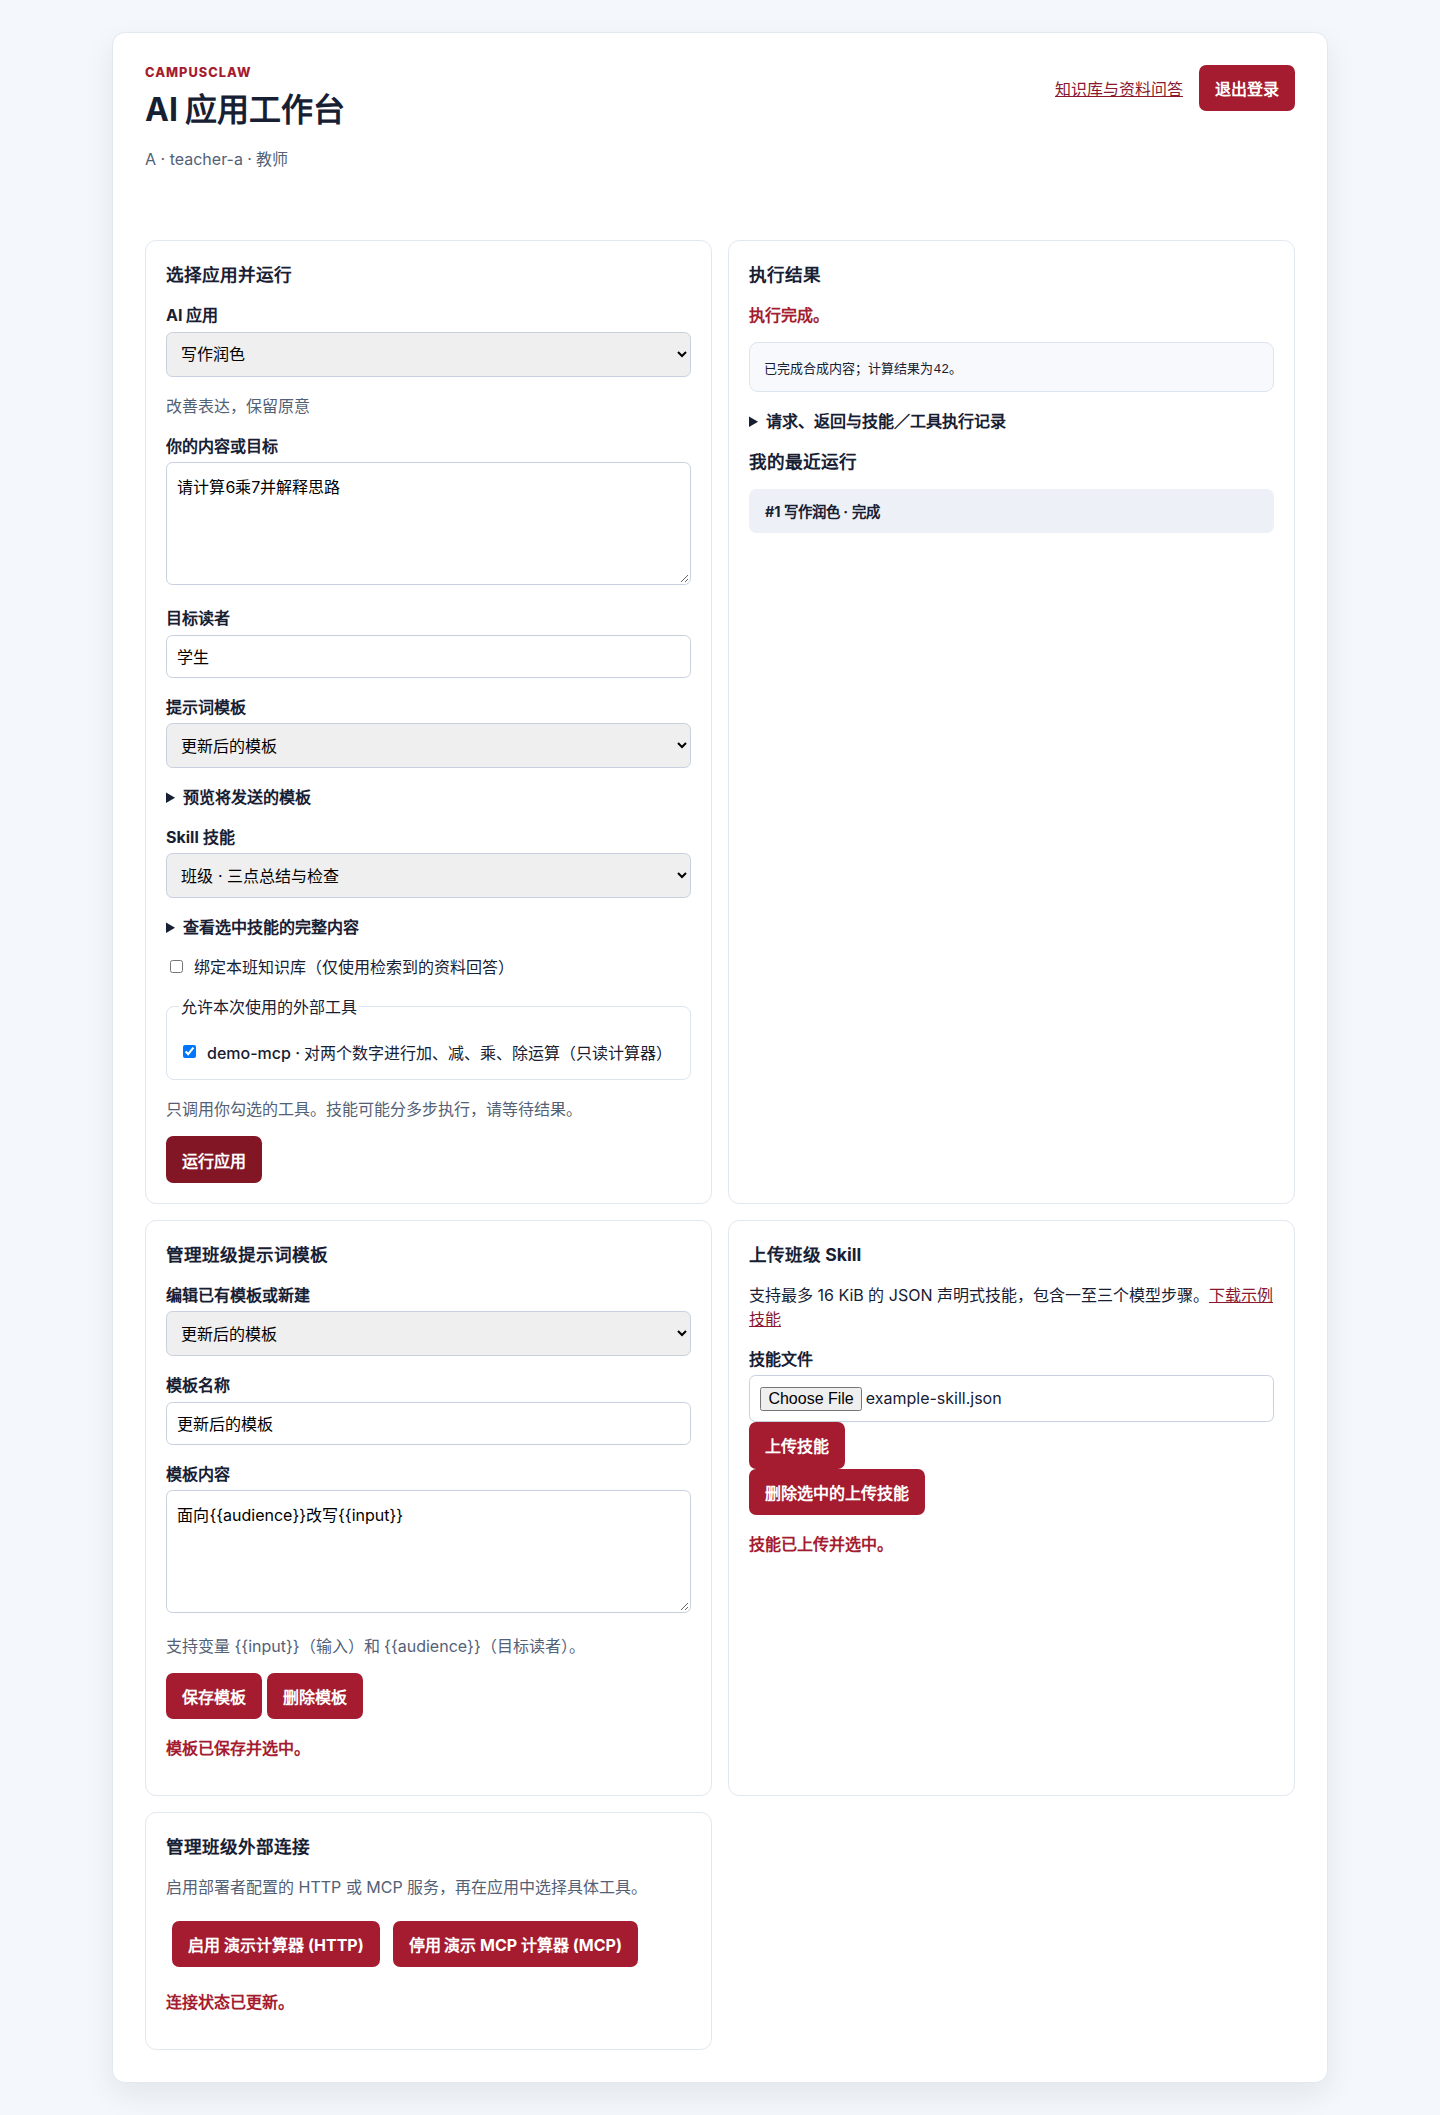
\includegraphics[width=0.94\linewidth,height=0.67\textheight,keepaspectratio]{docs/verification/workspace.png}
\end{center}
\textbf{已完成：}五类能力均有用户可操作入口、服务端实现和测试/调用证据，已部署到现有服务。报告不将仅写入配置、仅显示名称或忽略参数判作技能/工具执行成功。

\textbf{使用边界：}上传技能采用明确的 JSON 模型步骤格式；MCP 限于已声明协议与传输范围；外部连接由部署者审批配置、教师启用、用户按次选择。需接入新的技能包格式、MCP 传输或额外业务流程时，应另建需求并验证。

\textbf{最终判定：个人 AI 应用平台在本次要求和已声明支持范围内通过验收。}后续直接复用已完成的平台能力，针对新的增量目标继续开发。
\end{document}
